\documentclass{beamer}


\usepackage{times,amsmath,amssymb,color,array}
\usepackage{algorithm,algorithmic}
\usepackage{listings}
\usepackage{tikz}
\usepackage{bm}

% -- document geometry (options available to specify page margins)
\usepackage{geometry}
%\usepackage[left=3cm,right=3cm,top=2.5cm,bottom=3.5cm]{geometry}

% -- support for graphics with epstopdf conversion
\ifx\pdfoutput\undefined
\usepackage{graphicx}
\else
\usepackage{graphicx}
\usepackage{epstopdf}
\fi
% -- graphics search path
\graphicspath{{images/}}

%% ========================================================
%% -- BEAMER --
%% ========================================================
\mode<presentation>
{
%   \usetheme{Goettingen}
%    \usetheme{Marburg}
    \setbeamercovered{transparent}
}
%\usepackage{beamerthemeshadow}
%\usepackage{beamerthemesplit}
% \AtBeginSubsection[] {
%     \begin{frame}<beamer>
%     \frametitle{Outline}
%     \tableofcontents[currentsection,currentsubsection]
%     \end{frame}
% }

% -- Set paragraph indentation and spacing
%\setlength{\parindent}{6mm}
%\setlength{\parskip}{3mm plus4mm minus3mm}

% -- number equations as sub-numbers of section
\numberwithin{figure}{section}
\numberwithin{equation}{section}

% -- specify depth of table of contents
\setcounter{tocdepth}{3}

% -- specify depth to which to number sections
\setcounter{secnumdepth}{2}

% -- specify style of bibliography
\bibliographystyle{plain}

% -- colours
\definecolor{CadetBlue}{rgb}{0.0,0,0.55} 
\definecolor{Black}{rgb}{0.0,0,0.0} 
\definecolor{OliveGreen}{rgb}{0.0,0.55,0.0} 
\definecolor{Brown}{rgb}{0.55,0.55,0.0} 

% -- configure lstlistings
% \lstset{frame=ltrb,framesep=3pt,basicstyle=\scriptsize,
%     keywordstyle=[1]\ttfamily\color{CadetBlue},
%     identifierstyle=\ttfamily\color{Black}\bfseries,
%     commentstyle=\color{OliveGreen},
%     stringstyle=\color{Brown}\ttfamily,
%     showstringspaces=false
% }
\lstset{language=Java,captionpos=t,tabsize=3,frame=no,keywordstyle=\color{blue},
   commentstyle=\color{gray},identifierstyle=\color{OliveGreen},stringstyle=\color{red},numberstyle=\tiny,
   numbersep=5pt,breaklines=true,showstringspaces=false,basicstyle=\footnotesize,emph={label}}

    \pgfdeclarelayer{background}
    \pgfdeclarelayer{foreground}
    \pgfsetlayers{background,main,foreground}

%\renewcommand{\frametitle}[1]{\begin{center}\Large\bf #1\end{center}}

% ============================================================================
\title{Nektar++: Technical Introduction}
\author{\includegraphics[width=0.5\textwidth,trim=10mm 70mm 15mm 40mm,clip]
{title.pdf}\\Chris Cantwell}
%\institute{Imperial College London}
\subject{Spectral/$hp$ element methods}
\logo{\includegraphics[height=0.75cm]{imperial}}
\date{7th February 2011}

\begin{document}

\frame{\titlepage}


\begin{frame}
\frametitle{Nektar++: A Technical Introduction}
\begin{minipage}[c][0.8\textheight][t]{\linewidth}
\begin{itemize}
  \item Aim to introduce the \emph{Nektar++} library and demonstrate its use in
  practice.
  \item Outline
  \bigskip
  \begin{itemize}
  \item Define the problem
  \begin{itemize}
    \item Mesh Definition
    \item Nektar++ XML file format
  \end{itemize}
  \item Solving the problem
  \begin{itemize}
    \item Basic ingredients
    \item Helmholtz equation in 2D
    \item Unsteady Advection-Diffusion
  \end{itemize}
  \end{itemize}
  \bigskip
  \item Hands-on tutorial.
\end{itemize}
\bigskip
\bigskip
Useful prerequisites: C/C++
\end{minipage}
\end{frame}

\begin{frame}
\frametitle{Mesh Definition}
\begin{minipage}[c][0.8\textheight][t]{\linewidth}
\begin{columns}
\begin{column}[l]{7cm}
    Mesh defined in terms of:
    \begin{itemize}
      \item Vertices
      \item Edges
      \item Elements
    \end{itemize}
    \bigskip
    Support for a range of elements:
    \begin{itemize}
      \item 1D: Segment
      \item 2D: Triangle, Quadrilateral
      \item 3D: Tetrahedron, Hexahedron
    \end{itemize}
\end{column}
\begin{column}[l]{4cm}
    \includegraphics[width=\textwidth]{mesh}
\end{column}
\end{columns}
    \bigskip
    Mesh definition specified using XML.
\end{minipage}
\end{frame}

\begin{frame}[fragile]
\frametitle{XML file}
\begin{minipage}[c][0.8\textheight][t]{\linewidth}
\begin{columns}
\begin{column}[l]{11.5cm}
\begin{itemize}
\item e\textbf{X}tensible \textbf{M}arkup \textbf{L}anguage - similar concept to
HTML.
\item A hierarchial document
\begin{itemize}
  \item tags (XML 'elements'), attributes, content.
\end{itemize}

\end{itemize}

\begin{center}
\begin{lstlisting}
  <VERTEX>
    <V ID="0"> 0.1 1.0 0.0 </V>
  </VERTEX>
\end{lstlisting}
\end{center}
\begin{itemize}
  \item Open tag with \lstinline{<NAME>}
  \item Close tag with matching \lstinline{</NAME>}
  \item Each tag has a name (no uniqueness requirement)
  \item Each tag may contain one of more attributes
  (\lstinline{ID="0"})
  \item Each tag may contain element text
  \lstinline{<V...> 0.1  1.0  0.0 </V>}
  \item \ldots or other elements (\lstinline{<VERTEX><V>...</V></VERTEX})
\end{itemize}
\end{column}
\end{columns}
\end{minipage}
\end{frame}

\begin{frame}[fragile]
\frametitle{XML file}
\begin{minipage}[c][0.8\textheight][t]{\linewidth}
\begin{lstlisting}
<NEKTAR>
    <GEOMETRY DIM="1" SPACE="2">
        <VERTEX>
            ...
        </VERTEX>
        <ELEMENT>
            ...
        </ELEMENT>
        <COMPOSITE>
            ...
        </COMPOSITE>
        <DOMAIN> C[0] </DOMAIN>
    </GEOMETRY>
    <EXPANSIONS>
      <E COMPOSITE="C[0]" NUMMODES="8" TYPE="MODIFIED"/>
    </EXPANSIONS>
    <CONDITIONS>
      ...
    </CONDITONS>
</NEKTAR>
\end{lstlisting}
\end{minipage}
\end{frame}


\begin{frame}[fragile]
\frametitle{Mesh Definition}
\begin{minipage}[c][0.9\textheight][t]{\linewidth}
\begin{columns}
\begin{column}[l]{7cm}
\begin{itemize}
  \item Each component has unique index
  \item Tag name specifies component type
  \item Each vertex has 3 coordinates
  \begin{lstlisting}
<V ID="0"> 0.5 1.0 0.0 </V>
  \end{lstlisting}
  \item Edges defined by two vertices
  \begin{lstlisting}
<E ID="0"> 3 6 </E>
  \end{lstlisting}
  (We also define faces in 3D)
  \item Elements defined by set of edges (2D) or faces (3D)
  \begin{lstlisting}
<T ID="0">   4  5  6    </T>
<Q ID="20"> 17 18 21 20 </Q>
  \end{lstlisting}
  \item Composites define groups of entities
  \begin{lstlisting}
<C ID="0"> Q[0-4] </C>
<C ID="1"> E[0-8] </C>
  \end{lstlisting}
\end{itemize}
\end{column}
\begin{column}[l]{4cm}
\vspace{-20mm}
    \includegraphics[width=\textwidth]{mesh}\\
  Element types (tag names):
  \begin{itemize}
  \item Segment(\lstinline{<S>})
  \item Triangle (\lstinline{<T>})
  \item Quadrilateral(\lstinline{<Q>}) 
  \item Tetrahedron(\lstinline{<A>}) 
  \item Hexahedron(\lstinline{<H>})
  \end{itemize}
\end{column}
\end{columns}

\end{minipage}
\end{frame}


\begin{frame}[fragile]
\frametitle{Mesh Generation}
\begin{minipage}[c][0.8\textheight][t]{\linewidth}
\begin{columns}
\begin{column}[l]{7cm}
\begin{itemize}
  \item Define geometry in GMSH
  \begin{lstlisting}
  ...
  Point(1) = {0,0,0};
  Line(1) = {16,29};
  Line Loop(54) = {1,-18,-17,16};
  Plane Surface(54) = {54};
  ...
  \end{lstlisting}
  \item Generate mesh
  \begin{verbatim}
  gmsh -2 example.geo
  \end{verbatim}\vspace{-5mm}
  \item Translate mesh
  \begin{verbatim}
  MeshConvert example.msh \
     example.xml
  \end{verbatim}\vspace{-5mm}
  \item Fill in boundary conditions, etc
\end{itemize}
\end{column}
\begin{column}[r]{4cm}
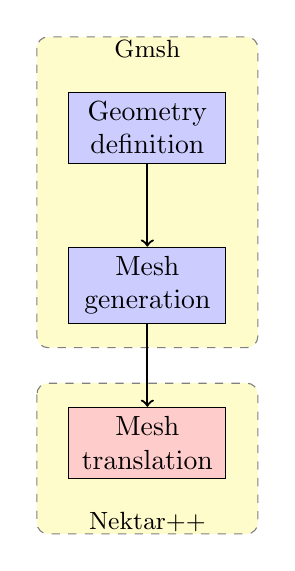
\begin{tikzpicture}
    \tikzstyle{box}=[draw, fill=blue!20, text width=5em, 
        text centered, minimum height=2.5em]
    \tikzstyle{ann} = [above, text width=5em]

    \node[box] (geom) at (0,0) {Geometry definition};
    \node[above of=geom] (gmsh) {\small{Gmsh}};
    \node[box] (mesh-gen) at (0,-2) {Mesh generation};
    \draw[->,thick] (geom) -- (mesh-gen);
    \node[box,fill=red!20] (mesh-trans) at (0,-4) {Mesh translation};
    \node[below of=mesh-trans] (nektar) {\small{Nektar++}};
    \draw[->,thick] (mesh-gen) -- (mesh-trans);
    \begin{pgfonlayer}{background}
        \path (geom.west |- geom.north)+(-0.4,0.7) node (a) {};
        \path (mesh-gen.south -| mesh-gen.east)+(+0.4,-0.3) node (b) {};
        \path[fill=yellow!20,rounded corners, draw=black!50, dashed]
            (a) rectangle (b);
        \path (mesh-trans.west |- mesh-trans.north)+(-0.4,0.3) node (a) {};
        \path (mesh-trans.south -| mesh-trans.east)+(+0.4,-0.7) node (b) {};
        \path[fill=yellow!20,rounded corners, draw=black!50, dashed]
            (a) rectangle (b);
    \end{pgfonlayer}
\end{tikzpicture}
\end{column}
\end{columns}
\end{minipage}

\end{frame}

\lstset{language=C++,basicstyle=\scriptsize,
    keywordstyle=[1]\ttfamily\color{CadetBlue},
    identifierstyle=\ttfamily\color{Black}\bfseries,
    commentstyle=\color{OliveGreen},
    stringstyle=\color{Brown}\ttfamily,
    showstringspaces=false
}

\begin{frame}[fragile]
\frametitle{Using Nektar++: Basic Ingredients in 2D}
\begin{minipage}[c][0.8\textheight][t]{\linewidth}
\begin{columns}
\begin{column}[l]{11.5cm}
Some principle components for using the Nektar++ framework:
\begin{itemize}
  \item Geometry and expansions definition (SpatialDomains)
  \begin{lstlisting}
  SpatialDomains::MeshGraph2D graph2D;
  graph2D.ReadGeometry("example.xml");
  graph2D.ReadExpansions("example.xml");
  \end{lstlisting}
  \item Boundary conditions (SpatialDomains)
  \begin{lstlisting}
  SpatialDomains::BoundaryConditions bcs(&graph2D);
  bcs.Read("example.xml");
  \end{lstlisting}
  \item Continuous Galerkin solution field (MultiRegions)
  \begin{lstlisting}
  MultiRegions::ContField2DSharedPtr Exp;
  Exp = MemoryManager<MultiRegions::ContField2D>::
                AllocateSharedPtr(graph2D,bcs);
  \end{lstlisting}
  \textbf{OR} Discontinuous Galerkin solution field (MultiRegions)
  \begin{lstlisting}
  MultiRegions::DisContField2DSharedPtr Exp;
  Exp = MemoryManager<MultiRegions::DisContField2D>::
                AllocateSharedPtr(graph2D,bcs);
  \end{lstlisting}
\end{itemize}
\end{column}
\end{columns}
\end{minipage}
\end{frame}

\lstset{language=Java,captionpos=t,tabsize=3,frame=no,keywordstyle=\color{blue},
   commentstyle=\color{gray},identifierstyle=\color{OliveGreen},stringstyle=\color{red},numberstyle=\tiny,
   numbersep=5pt,breaklines=true,showstringspaces=false,basicstyle=\scriptsize,emph={label}}

\begin{frame}[fragile]
\frametitle{Using Nektar++: Helmholtz2D Demo}
\begin{minipage}[c][0.8\textheight][t]{\linewidth}
\begin{columns}
\begin{column}[l]{6cm}
Solve Helmholtz problem 
\begin{align*}
    \nabla^2 u - \lambda u = f.
\end{align*}
\vspace{-7mm}
\begin{itemize}
  \item Forcing function:
  \begin{align*}
  f = -(\lambda + 2\pi^2)\sin(\pi x)\sin(\pi y)
  \end{align*}
  \item Analytic solution:
  \begin{align*}
  u = \sin(\pi x)\sin(\pi y)
  \end{align*}
\end{itemize}
\end{column}
\begin{column}[r]{5cm}
\includegraphics[width=\textwidth]{Test_HEL}
\end{column}
\end{columns}
\vspace{3mm}
Specifying forcing and analytic solution:
  \begin{lstlisting}
<FORCING>
  <F VAR="u" VALUE="-(Lambda + 2*PI*PI)*sin(PI*x)*sin(PI*y)" />
</FORCING>

<EXACTSOLUTION>
  <F VAR="u" VALUE="sin(PI*x)*sin(PI*y)" />
</EXACTSOLUTION>
  \end{lstlisting}
\end{minipage}
\end{frame}


\begin{frame}[fragile]
\frametitle{Using Nektar++: Boundary Conditions}
\begin{minipage}[c][0.8\textheight][t]{\linewidth}
\begin{columns}
\begin{column}[l]{11.5cm}
\begin{itemize}
  \item Use composite to select boundary mesh elements
  \begin{lstlisting}
<C ID="1"> E[0,31,3,32,38,39,11,12,22]</C>
  \end{lstlisting}
  \item Define boundary regions using these composites
  \begin{lstlisting}
<BOUNDARYREGIONS>
  <B ID="0"> C[1] </B>
</BOUNDARYREGIONS>
  \end{lstlisting}
  \item Define type and value for each boundary region
  \begin{lstlisting}
<BOUNDARYCONDITIONS>
  <REGION REF="0">
    <D VAR="u" VALUE="sin(PI*x)*sin(PI*y)" />
  </REGION>
</BOUNDARYCONDITIONS>
  \end{lstlisting}
  \item Types: Dirichlet(\texttt{D}), Neumann(\texttt{N})
%   \item Support for high-order pressure BC 
%   (\lstinline{USERDEFINEDTYPE="H"})
%   \item Support for time-dependent BC
%   (\lstinline{USERDEFINEDTYPE="TimeDependent"})
\end{itemize}
\end{column}
\end{columns}
\end{minipage}
\end{frame}


\lstset{language=C++,basicstyle=\scriptsize,
    keywordstyle=[1]\ttfamily\color{CadetBlue},
    identifierstyle=\ttfamily\color{Black}\bfseries,
    commentstyle=\color{OliveGreen},
    stringstyle=\color{Brown}\ttfamily,
    showstringspaces=false
}

\begin{frame}[fragile]
\frametitle{Using Nektar++: Helmholtz2D Demo}
\begin{minipage}[c][0.8\textheight][t]{\linewidth}
\begin{columns}
\begin{column}[l]{11.5cm}
\begin{itemize}
  \item Read in forcing function
  \begin{lstlisting}
  Array<OneD,NekDouble> fce = Array<OneD,NekDouble>(nq);
  SpatialDomains::ConstForcingFunctionShPtr ffunc
            = bcs.GetForcingFunction(bcs.GetVariable(0));
  \end{lstlisting}
  \item \ldots evaluate it at each quadrature point\ldots
  \begin{lstlisting}
  for(i = 0; i < nq; ++i)
  {
      fce[i] = ffunc->Evaluate(x[i],y[i],z[i]);
  }
  \end{lstlisting}
  \item \ldots and create a corresponding solution field on the same mesh
  \begin{lstlisting}
  MultiRegions::ContField2DSharedPtr Fce;
  Fce = MemoryManager<MultiRegions::ContField2D>::
                AllocateSharedPtr(*Exp);
  Fce->SetPhys(fce);
  \end{lstlisting}
\end{itemize}
\end{column}
\end{columns}
\end{minipage}
\end{frame}


\begin{frame}[fragile]
\frametitle{Using Nektar++: Helmholtz2D Demo}
\begin{minipage}[c][0.8\textheight][t]{\linewidth}
\begin{columns}
\begin{column}[l]{11.5cm}
\begin{itemize}
  \item Finally, we solve for $\hat{u}$
  \begin{lstlisting}
  Exp->HelmSolve( Fce->GetPhys(), 
                  Exp->UpdateContCoeffs(), 
                  lambda, 
                  true);
  \end{lstlisting}
  \item \ldots and transform back into physical space $u$
  \begin{lstlisting}
  Exp->BwdTrans(  Exp->GetContCoeffs(), 
                  Exp->UpdatePhys(), 
                  true);
  \end{lstlisting}
\end{itemize}
\end{column}
\end{columns}
\end{minipage}
\end{frame}

\begin{frame}[fragile]
\frametitle{Using Nektar++: Helmholtz2D Demo}
\begin{minipage}[c][0.8\textheight][t]{\linewidth}
\begin{columns}
\begin{column}[l]{11.5cm}
Run \texttt{Helmholtz2D}:
\begin{verbatim}
./Helmholtz2D Test_HEL.xml
\end{verbatim}
\ldots and visualise output.
\end{column}
\end{columns}
\end{minipage}
\end{frame}

% \begin{frame}[fragile]
% \frametitle{Using Nektar++: Unsteady Advection-Diffusion}
% \begin{minipage}[c][0.8\textheight][t]{\linewidth}
% \begin{columns}
% \begin{column}[l]{11.5cm}
% \begin{align*}
%     \frac{\partial u}{\partial t} + \frac{\partial u}{\partial x}
%             = \frac{\partial^2 u}{\partial x^2}
% \end{align*}
% \begin{itemize}
%   \item Weak form:
%   $(v,\frac{\partial u}{\partial t}) + (v,\frac{\partial
%   u}{\partial x}) = (v,\frac{\partial^2 u}{\partial x^2})$
%   \item Semi-discrete representation:
%   $\bm{M}\frac{d\bm{\hat{u}}}{dt} + \bm{A\hat{u}} = \bm{L\hat{u}}$
%   \item 
% \end{itemize}
% \end{column}
% \end{columns}
% \end{minipage}
% \end{frame}
% 
% 
% \begin{frame}[fragile]
% \frametitle{Using Nektar++: Time Integration}
% \begin{minipage}[c][0.8\textheight][t]{\linewidth}
% \begin{columns}
% \begin{column}[l]{11.5cm}
% A framework for time integration:
% \begin{itemize}
%   \item Need four components
%   \begin{lstlisting}
%   LibUtilities::TimeIntegrationSchemeOperators   m_ode;
%   LibUtilities::TimeIntegrationSchemeKey         IntKey;
%   LibUtilities::TimeIntegrationSchemeSharedPtr   IntScheme;
%   LibUtilities::TimeIntegrationSolutionSharedPtr u;
%   \end{lstlisting}
%   \item Choose a scheme to use
%   \begin{lstlisting}
%   IntKey = TimeIntegrationSchemeKey(eClassicalRungeKutta4);
%   \end{lstlisting}
%   \item Define an ODE using two functions
%   \begin{lstlisting}
%   m_ode.DefineImplicitSolve (&MyClass::DoImplicitSolve, this);
%   m_ode.DefineOdeRhs        (&MyClass::DoOdeRhs,        this);
%   \end{lstlisting}
%   \item Create and initialise the scheme
%   \begin{lstlisting}
%   IntScheme 
%        = LibUtilities::TimeIntegrationSchemeManager()[IntKey];
%   u = IntScheme->InitializeScheme( m_timestep, fields,
%                                    m_time, m_ode);
%   \end{lstlisting}
% \end{itemize}
% \end{column}
% \end{columns}
% \end{minipage}
% \end{frame}
% 
% \begin{frame}[fragile]
% \frametitle{Using Nektar++: Time Integration}
% \begin{minipage}[c][0.8\textheight][t]{\linewidth}
% \begin{columns}
% \begin{column}[l]{11.5cm}
% \begin{itemize}
%   \item Integrate in time
%   \begin{lstlisting}
%   for(n = 0; n < m_steps; ++n) 
%   {
%     fields =  IntScheme->TimeIntegrate(m_timestep,u,m_ode);
%     m_time += m_timestep;
%   }
%   \end{lstlisting}
%   \item Write out final output
%   \begin{lstlisting}
%   for(i = 0; i < nvariables; ++i)
%   {
%     m_fields[i]->UpdatePhys() = fields[i];
%   }
%   \end{lstlisting}
% \end{itemize}
% \end{column}
% \end{columns}
% \end{minipage}
% \end{frame}


\lstset{language=Java,captionpos=t,tabsize=3,frame=no,keywordstyle=\color{blue},
   commentstyle=\color{gray},identifierstyle=\color{OliveGreen},stringstyle=\color{red},numberstyle=\tiny,
   numbersep=5pt,breaklines=true,showstringspaces=false,basicstyle=\scriptsize,emph={label}}

\begin{frame}[fragile]
\frametitle{Using Nektar++: Advection-Diffusion-Reaction Solver}
\begin{minipage}[c][0.8\textheight][t]{\linewidth}
\begin{columns}
\begin{column}[l]{11.5cm}
\texttt{ADRSolver} provides a suite of solvers for a range of steady and
unsteady problems.
\begin{itemize}
  \item \texttt{Nektar++/solvers/ADRSolver}
  \item Additional session information needed:
  \begin{lstlisting}
<SOLVERINFO>
 <I PROPERTY="EQTYPE" VALUE="UnsteadyAdvectionDiffusion" />
 <I PROPERTY="Projection" VALUE="Continuous"/>
 
 <I PROPERTY="DiffusionAdvancement" VALUE="Implicit"/>
 <I PROPERTY="AdvectionAdvancement" VALUE="Explicit"/>
 
 <I PROPERTY="TimeIntegrationMethod" VALUE="IMEXOrder2"/>
</SOLVERINFO>
  \end{lstlisting}
  \item For unsteady problems, specify time integration parameters
  \begin{lstlisting}
<P> TimeStep      = 0.00001              </P>
<P> NumSteps      = 2000                 </P>

<P> IO_CheckSteps = 2000                 </P>
<P> IO_InfoSteps  = 2000                 </P>
  \end{lstlisting}
\end{itemize}
\end{column}
\end{columns}
\end{minipage}
\end{frame}


\begin{frame}[fragile]
\frametitle{Using Nektar++: Advection-Diffusion-Reaction Solver}
\begin{minipage}[c][0.8\textheight][t]{\linewidth}
\begin{columns}
\begin{column}[l]{11.5cm}
Run \texttt{ADRSolver}:
\begin{verbatim}
./ADRSolver Test_HEL.xml
\end{verbatim}
\end{column}
\end{columns}
\end{minipage}
\end{frame}


\begin{frame}[fragile]
\frametitle{Using Nektar++: Incompressible Navier-Stokes Solver}
\begin{minipage}[c][0.8\textheight][t]{\linewidth}
\begin{columns}
\begin{column}[l]{11.5cm}
\begin{itemize}
  \item \texttt{Nektar++/solvers/IncNavierStokesSolver}
  \item Support for high-order pressure and time-dependent boundary conditions
  \begin{lstlisting}
<BOUNDARYCONDITIONS>
  <REGION REF="0">
    <D VAR="u" USERDEFINEDTYPE="TimeDependent" 
          VALUE="-cos(x)*sin(y)*exp(-2*t*Kinvis)" />
    <D VAR="v" USERDEFINEDTYPE="TimeDependent" 
          VALUE="sin(x)*cos(y)*exp(-2*t*Kinvis)" />
    <N VAR="p" USERDEFINEDTYPE="H" VALUE="0"/>
  </REGION>
  <REGION REF="1">
    <D VAR="u" USERDEFINEDTYPE="TimeDependent" 
          VALUE="-cos(x)*sin(y)*exp(-2*t*Kinvis)" />
    <D VAR="v" USERDEFINEDTYPE="TimeDependent" 
          VALUE="sin(x)*cos(y)*exp(-2*t*Kinvis)" />
    <D VAR="p" USERDEFINEDTYPE="TimeDependent" 
          VALUE="-0.25*(cos(2*x)+cos(2*y))*exp(-4*t*Kinvis)"/>
  </REGION>
</BOUNDARYCONDITIONS>
  \end{lstlisting}
\end{itemize}
\end{column}
\end{columns}
\end{minipage}
\end{frame}

\begin{frame}[fragile]
\frametitle{Hands-on Tutorial}
\begin{minipage}[c][0.8\textheight][t]{\linewidth}
\begin{columns}
\begin{column}[l]{11.5cm}

\end{column}
\end{columns}
\end{minipage}
\end{frame}


\begin{frame}[fragile]
\frametitle{Further Information}
\begin{minipage}[c][0.8\textheight][t]{\linewidth}
\begin{columns}
\begin{column}[l]{11.5cm}
\begin{itemize} 
    \item \textbf{Nektar++ website}: \texttt{www.nektar.info}
    \begin{itemize}
      \item Example usage
      \item Educational Material
      \item Code documentation (Doxygen)
    \end{itemize}
    \item \textbf{Code Examples}: \texttt{Nektar++/library/Demos/}
    \item \textbf{Book}: \\
    {\scriptsize G.E. Karniadakis and S.J. Sherwin,
    \emph{Spectral/$hp$ element methods for computational fluid dynamics (2nd
    ed.)}, Oxford University Press (2005).}
    \item \textbf{Papers}:
    \begin{itemize}
      \item {\scriptsize\emph{A Generic Framework for Time-Stepping PDEs:
      general linear methods, object-orientated implementation and application
      to fluid problems}, Peter E.J. Vos, Sehun Chun, Alessandro Bolis, Claes
      Eskilsson, Robert M. Kirby and Spencer J. Sherwin , Int J. CFD, Submitted
      , 2011}
      \item {\scriptsize \ldots more on the website\ldots}\\
      {\scriptsize \texttt{http://www2.imperial.ac.uk/ssherw/spectralhp/pubs/}}
    \end{itemize}
\end{itemize}
\end{column}
\end{columns}
\end{minipage}
\end{frame}


\end{document}